
\documentclass{IEEEtran}
\usepackage{amsmath}
\usepackage{graphicx}
\author{Sumit Madhwani}
\title{Study on various Sorting Algorithms} 
\begin{document}
\maketitle


\begin{center}
Sorting Algorithms
\end{center}
A sorting algorithm is an algorithm that puts elements of a list in a certain order.Efficient sorting is important for optimizing the use of other algorithms (such as merge algorithm) which require input data to be in sorted lists.
\section{Selection Sort}
\subsection{pseudocode}
\begin{enumerate}
\item	    for j = 1 to n-1
\item	         smallest = j
\item		      	 for i = j + 1 to n
\item	                  if A[ i ] is less than A[ smallest ]
\item                          smallest = i
\item         	  Exchange A[ j ] with A[ smallest ]
\end{enumerate}

The algorithm divides the input list into two parts: the sublist of items already sorted, which is built up from left to right at the front (left) of the list, and the sublist of items remaining to be sorted that occupy the rest of the list. Initially, the sorted sublist is empty and the unsorted sublist is the entire input list. The algorithm proceeds by finding the smallest (or largest, depending on sorting order) element in the unsorted sublist, exchanging (swapping) it with the leftmost unsorted element (putting it in sorted order), and moving the sublist boundaries one element to the right.
 It has O(n*n) time complexity, 
\section{Bubble Sort}
Bubble sort, sometimes referred to as sinking sort, is a simple sorting algorithm that repeatedly steps through the list to be sorted, compares each pair of adjacent items and swaps them if they are in the wrong order. The pass through the list is repeated until no swaps are needed, which indicates that the list is sorted. The algorithm, which is a comparison sort, is named for the way smaller elements "bubble" to the top of the list. Although the algorithm is simple, it is too slow and impractical for most problems even when compared to insertion sort.[1] It can be practical if the input is usually in sorted order but may occasionally have some out-of-order elements nearly in position.
\section{Insertion Sort}
Insertion sort is a simple sorting algorithm that builds the final sorted array (or list) one item at a time. It is much less efficient on large lists than more advanced algorithms such as quicksort, heapsort, or merge sort.
\section{quick Sort}
Quicksort (sometimes called partition-exchange sort) is an efficient sorting algorithm, serving as a systematic method for placing the elements of an array in order. Developed by Tony Hoare in 1959,[1] with his work published in 1961,[2] it is still a commonly used algorithm for sorting. When implemented well, it can be about two or three times faster than its main competitors, merge sort and heapsort.[3]
\section{merge sort}
In computer science, merge sort (also commonly spelled mergesort) is an efficient, general-purpose, comparison-based sorting algorithm. Most implementations produce a stable sort, which means that the implementation preserves the input order of equal elements in the sorted output. Mergesort is a divide and conquer algorithm .


\begin{figure}
\section{\fontsize{10}{12}Number of comarisons in different sorting}
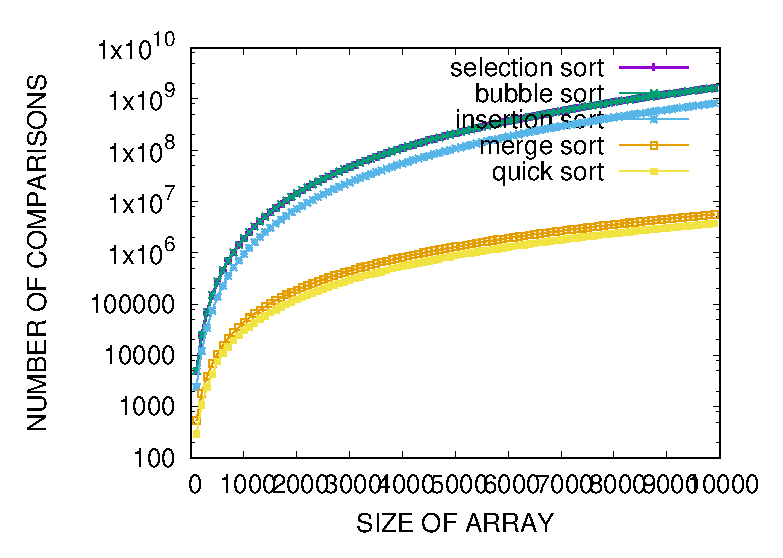
\includegraphics[width=6in]{comparison_graph.eps}
\section{Time taken in different sorting}
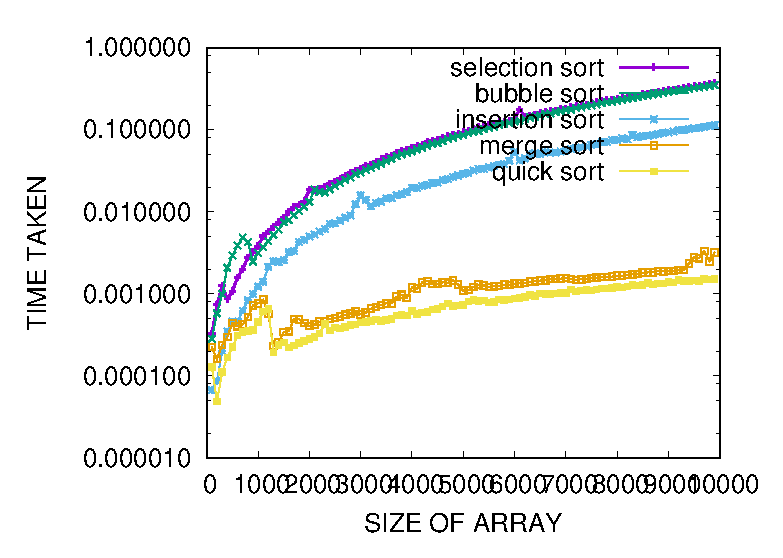
\includegraphics[width=6in]{time_graph.eps}
\end{figure} 




\end{document}

